% ----------------------------------------------------------------------

\newpage

\subsection{\phopt Test}
\label{ss:phoptimization}

\subsubsection{Purpose}

The \phopt test is responsible for setting an appropriate dynamic range for the 8-bit ADC that digitizes the recorded pulse height (PH).
The ADC is located in the Controller and Interface Block of the \roc.
It can be seen in the bottom right box of Figure~\ref{fig:puc}.
The two \dacs used to configure the ADC are \phoffset and \phscale.
\phoffset adds a constant offset to the pulse height measurement,
while \phscale effectively sets the gain of the ADC.
The \phopt test is designed to optimize these \dacs based on the most and least sensitive pixels in a given \roc.
There are two constraints used to simultaneously find a solution for \phoffset and \phscale.
First, the pixel with biggest pulse height reponse should saturate (PH = 255) at a user-defined signal strength
(default is \vcal = 100 (high range)).
Secondly, the pixel with the smallest pulse height response should have a reasonably large pulse height
(default is 20) at its \vcal turn-on threshold,
i.e. the lowest \vcal value for which the pixel fires.

\subsubsection{\textcolor{red}{Methodology}}
\subsubsection{Output}

% finding highest/lowest gain pixels

\begin{figure}[!Hp]
\centering
\begin{minipage}{0.45\textwidth}
  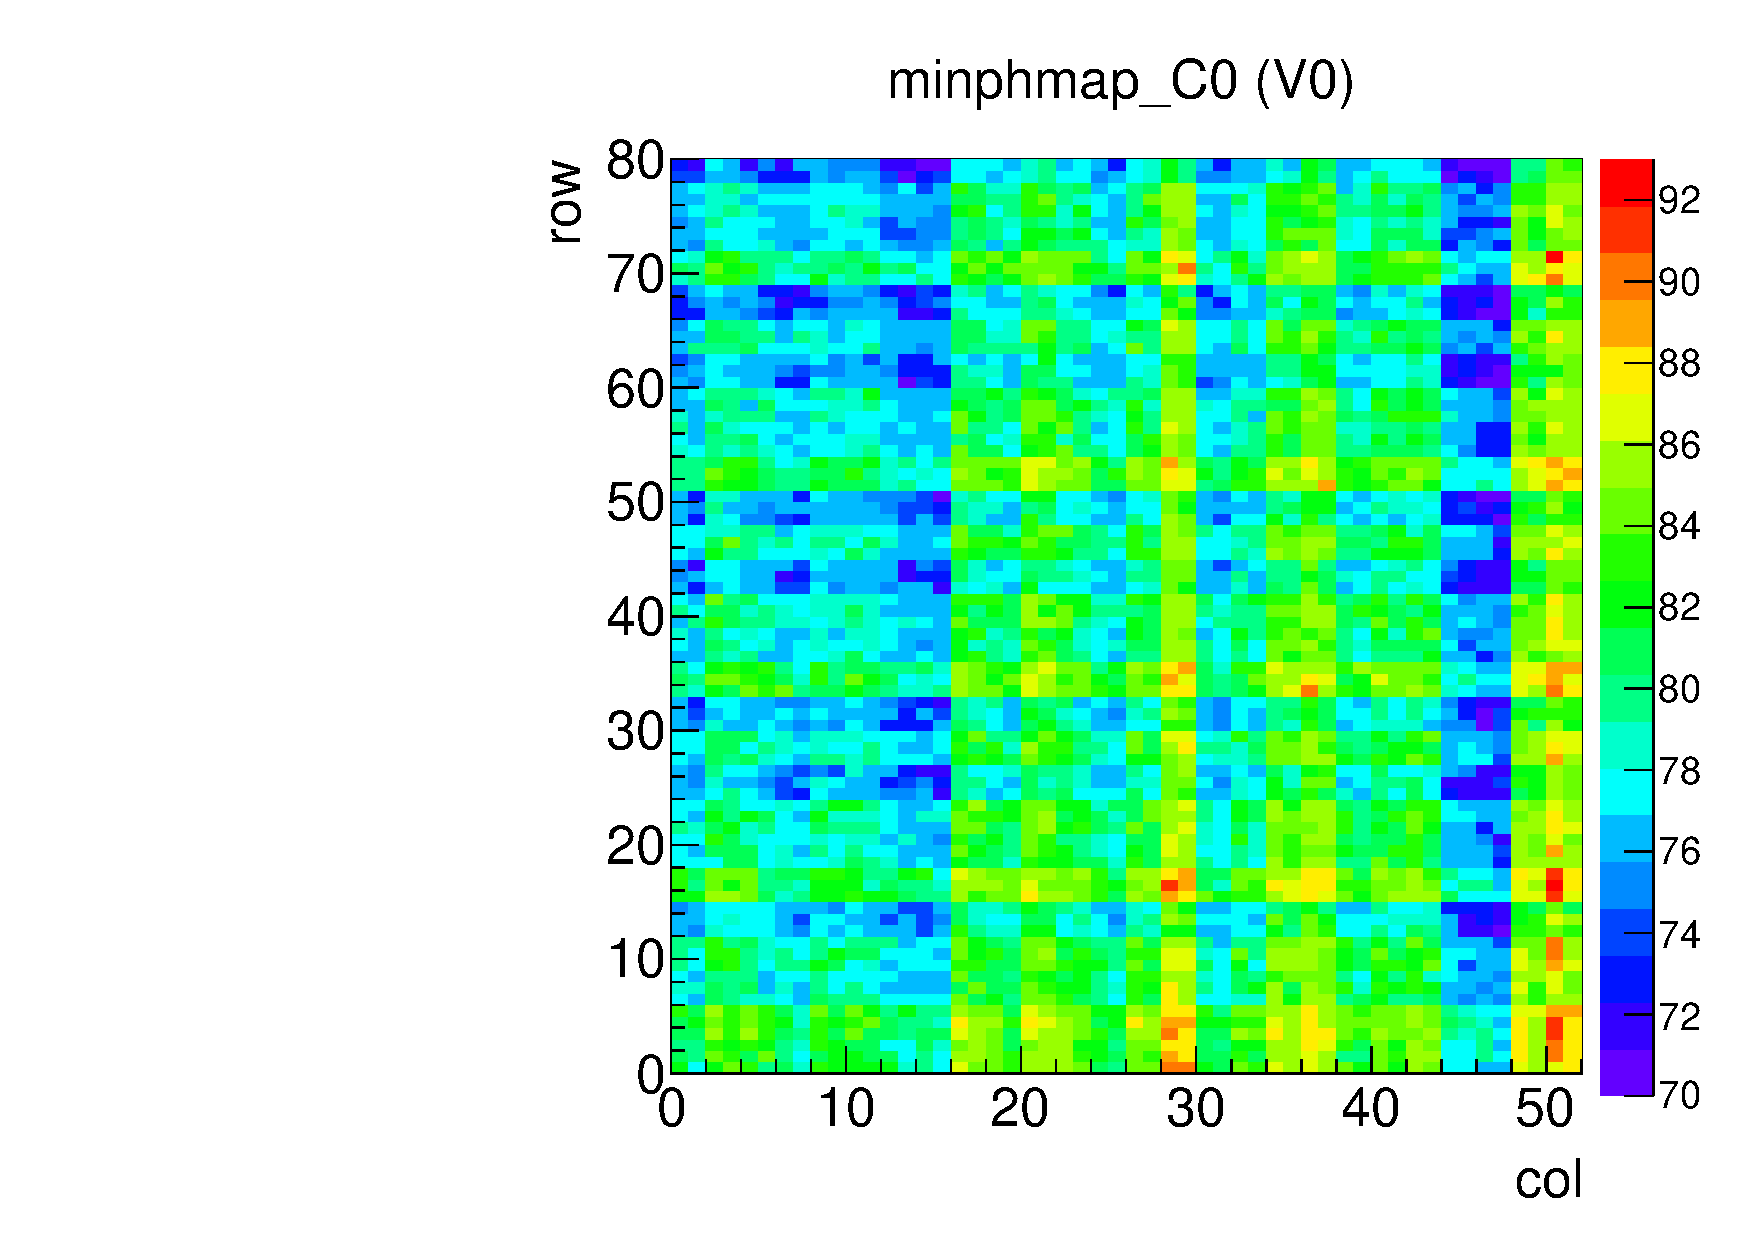
\includegraphics[width=1.0\textwidth]{figures/phopt_minphmap.pdf}
  \caption{}
  \label{fig:phopt_minphmap}
\end{minipage}
\hspace{0.3cm}
\begin{minipage}{0.45\textwidth}
  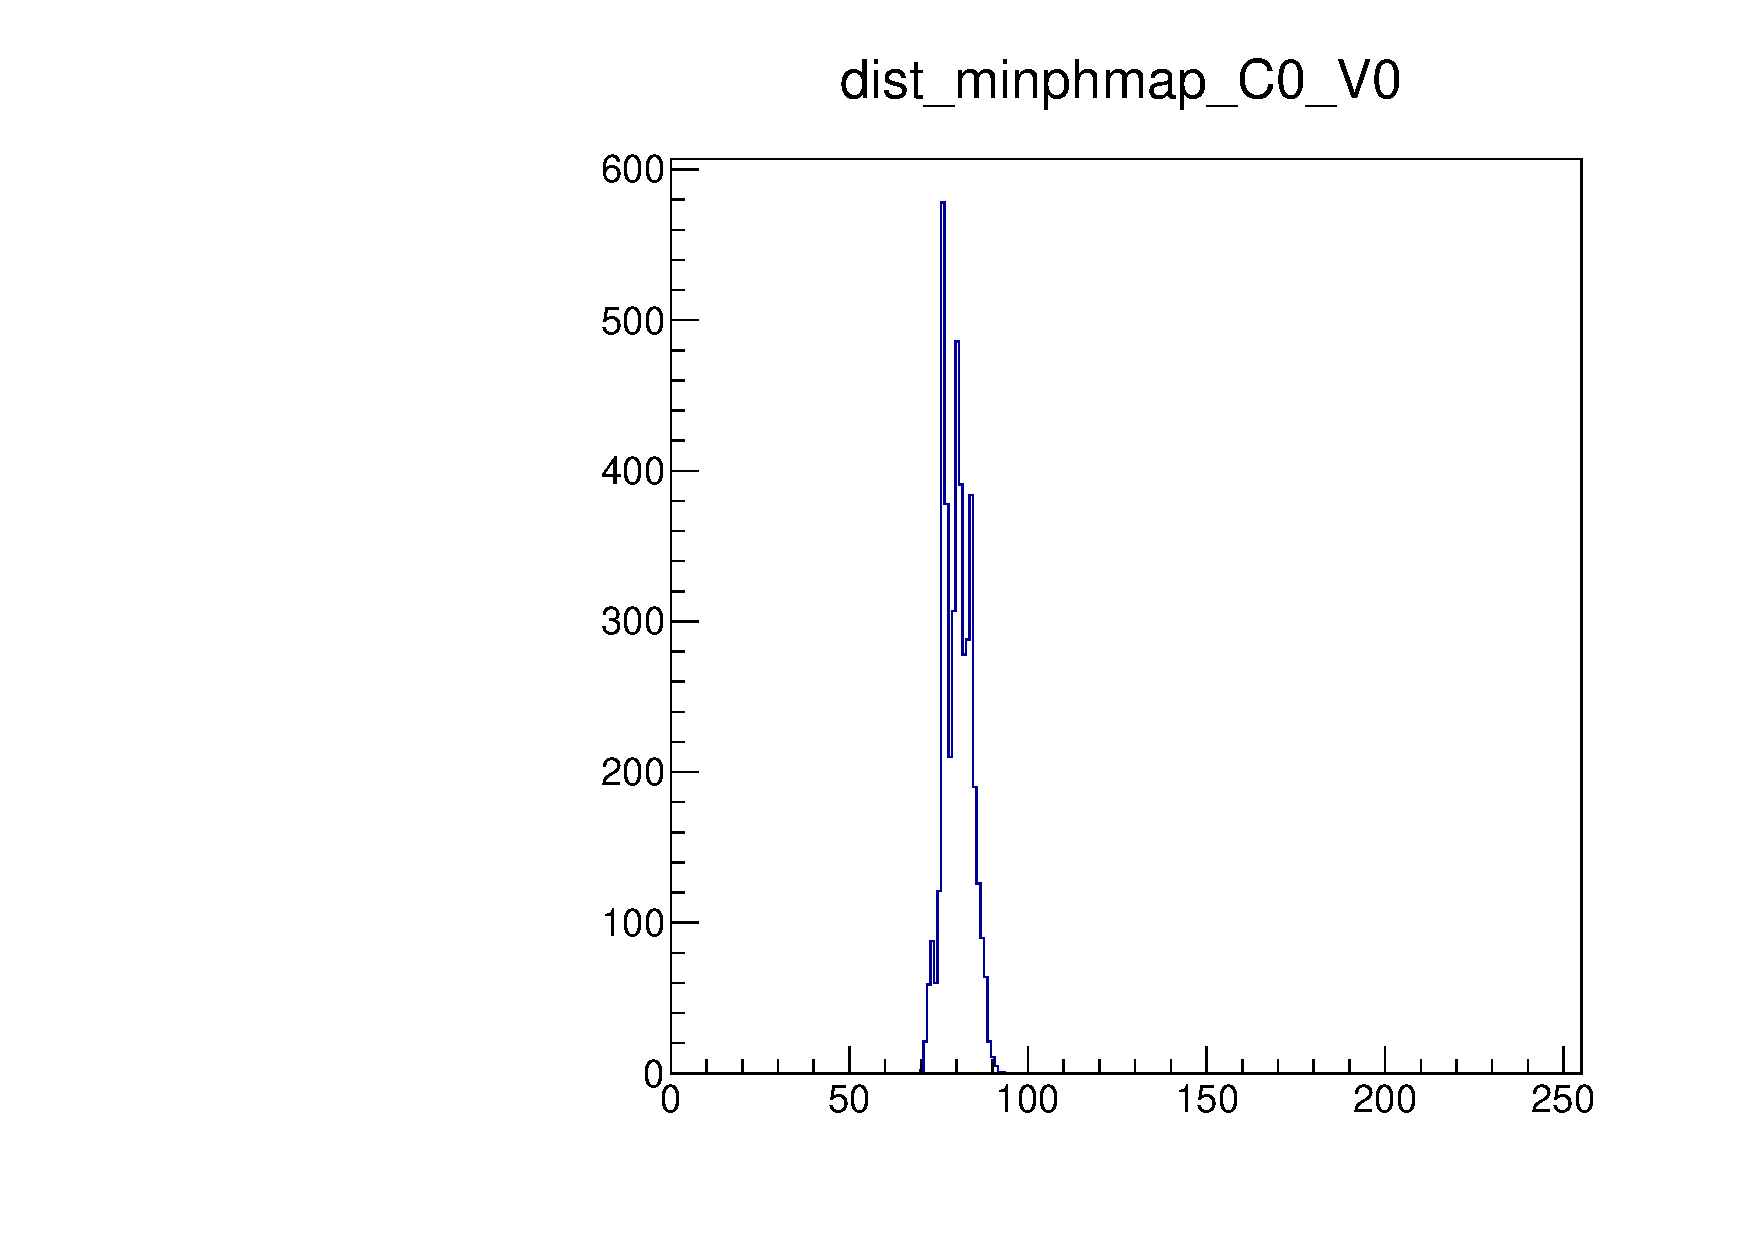
\includegraphics[width=1.0\textwidth]{figures/phopt_dist_minphmap.pdf}
  \caption{}
  \label{fig:phopt_dist_minphmap}
\end{minipage}
\end{figure}

\begin{figure}[!Hp]
\centering
\begin{minipage}{0.45\textwidth}
  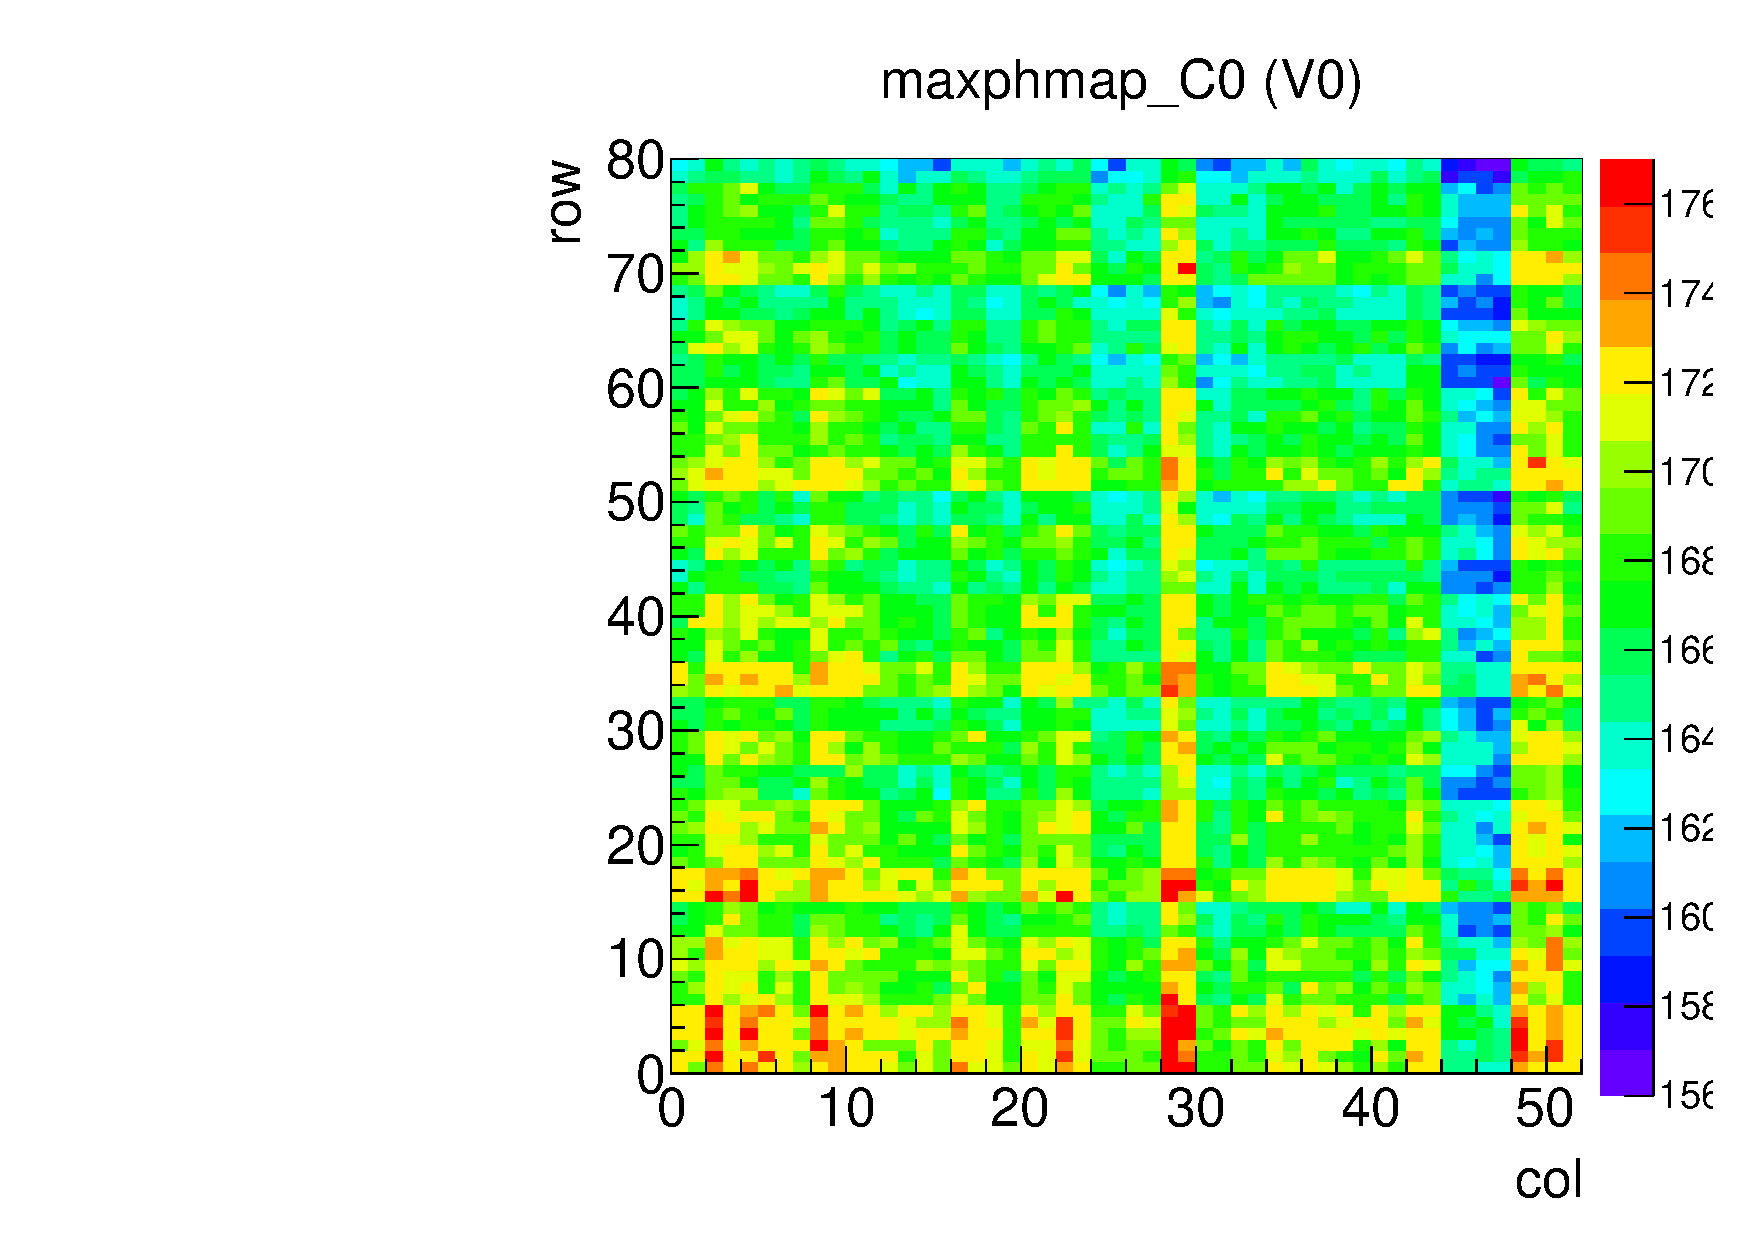
\includegraphics[width=1.0\textwidth]{figures/phopt_maxphmap.pdf}
  \caption{}
  \label{fig:phopt_maxphmap}
\end{minipage}
\hspace{0.3cm}
\begin{minipage}{0.45\textwidth}
  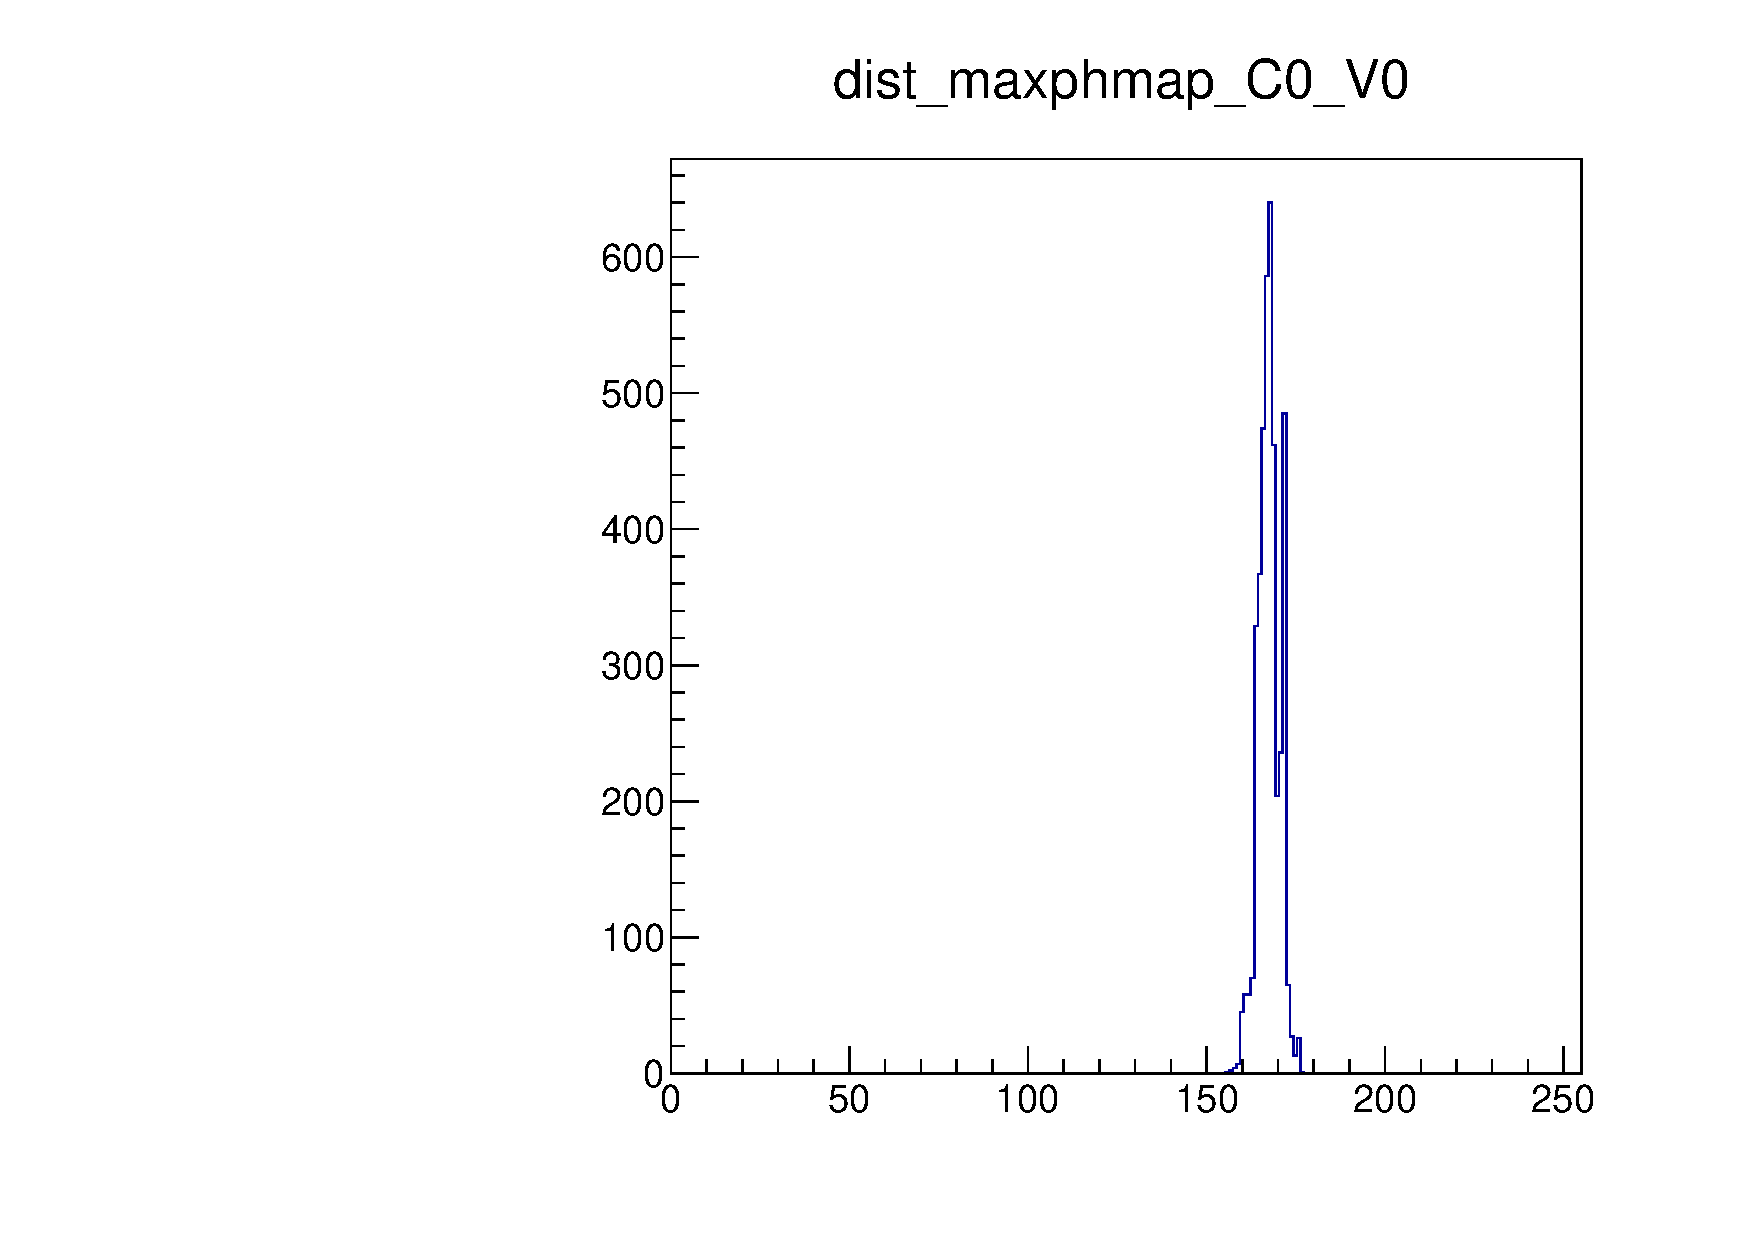
\includegraphics[width=1.0\textwidth]{figures/phopt_dist_maxphmap.pdf}
  \caption{}
  \label{fig:phopt_dist_maxphmap}
\end{minipage}
\end{figure}

% getting maps for optimization

\begin{figure}[!Hp]
\centering
\begin{minipage}{0.45\textwidth}
  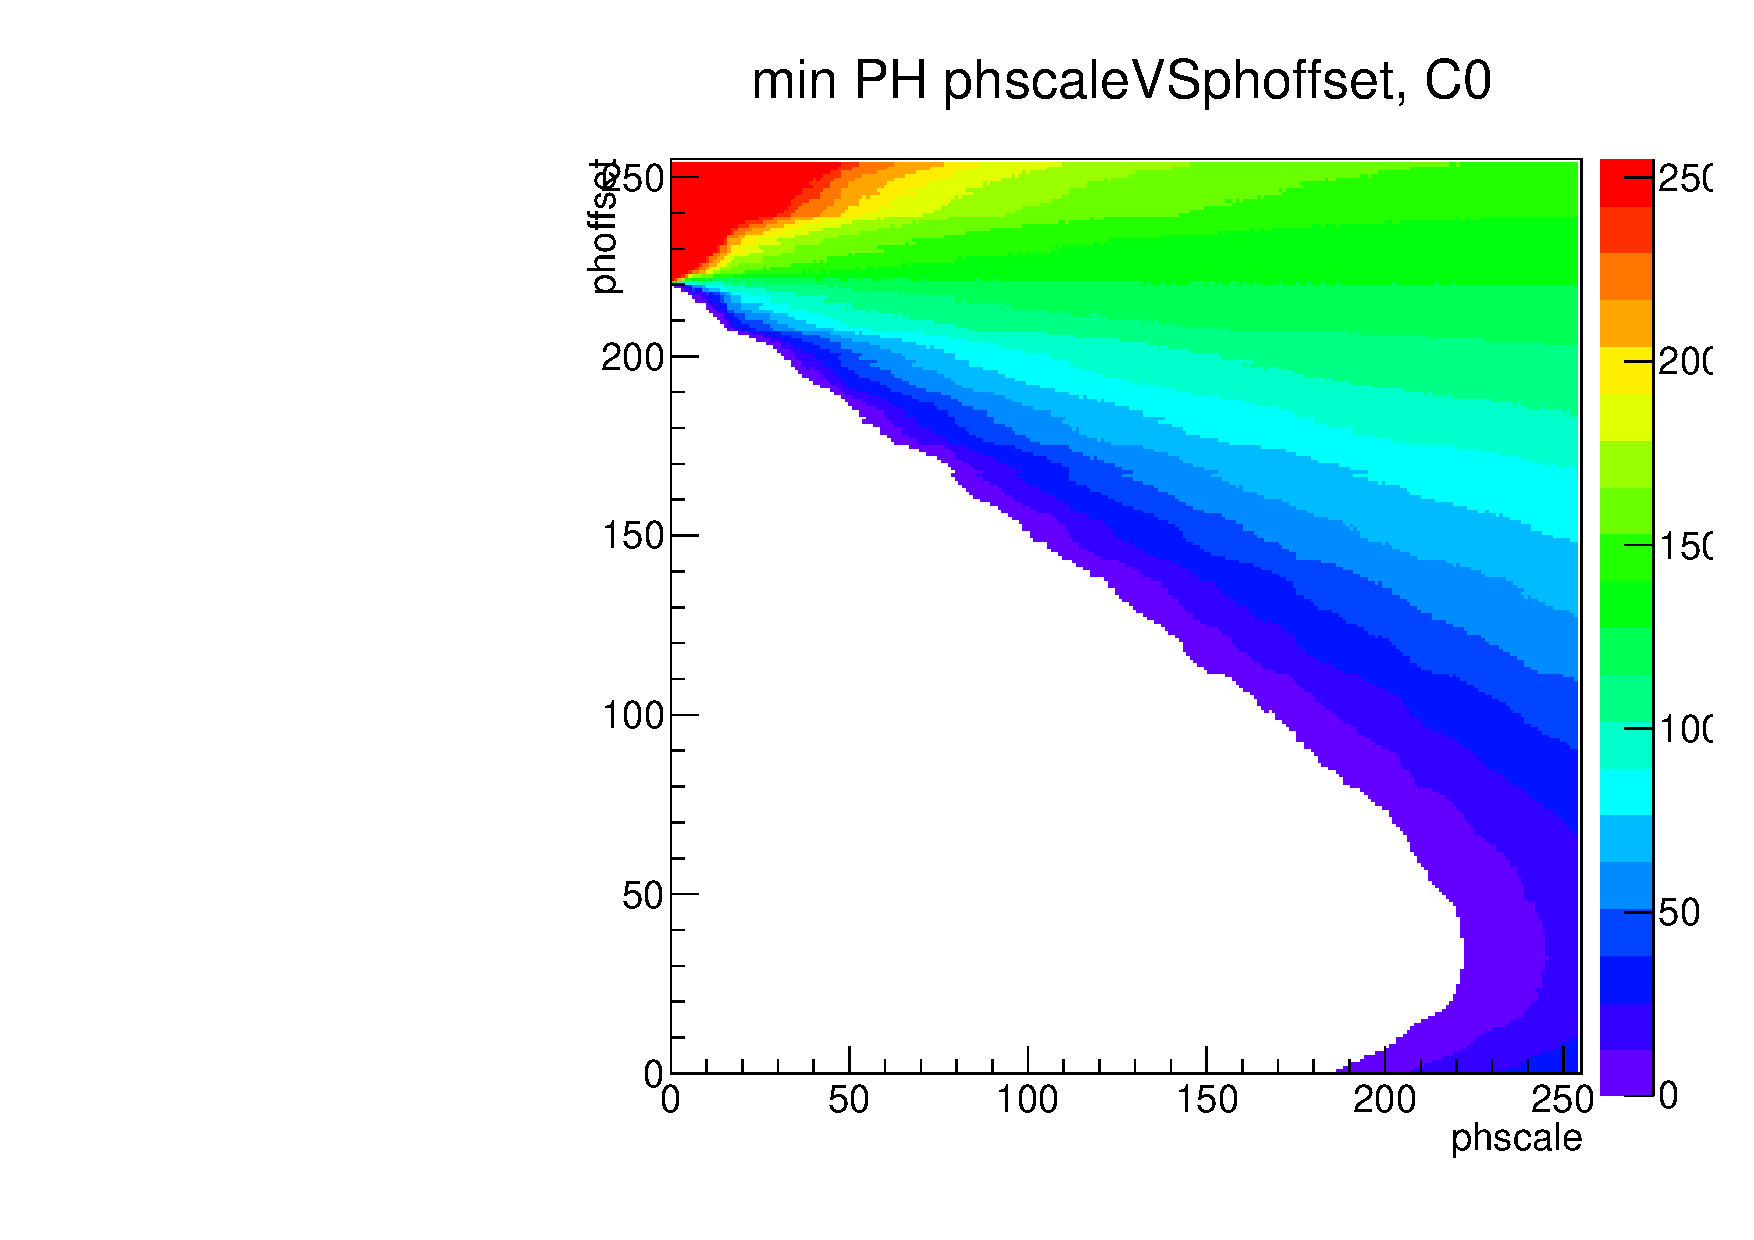
\includegraphics[width=1.0\textwidth]{figures/phopt_minphvsdacdac_th2.pdf}
  \caption{}
  \label{fig:phopt_minphvsdacdac_th2}
\end{minipage}
\hspace{0.3cm}
\begin{minipage}{0.45\textwidth}
  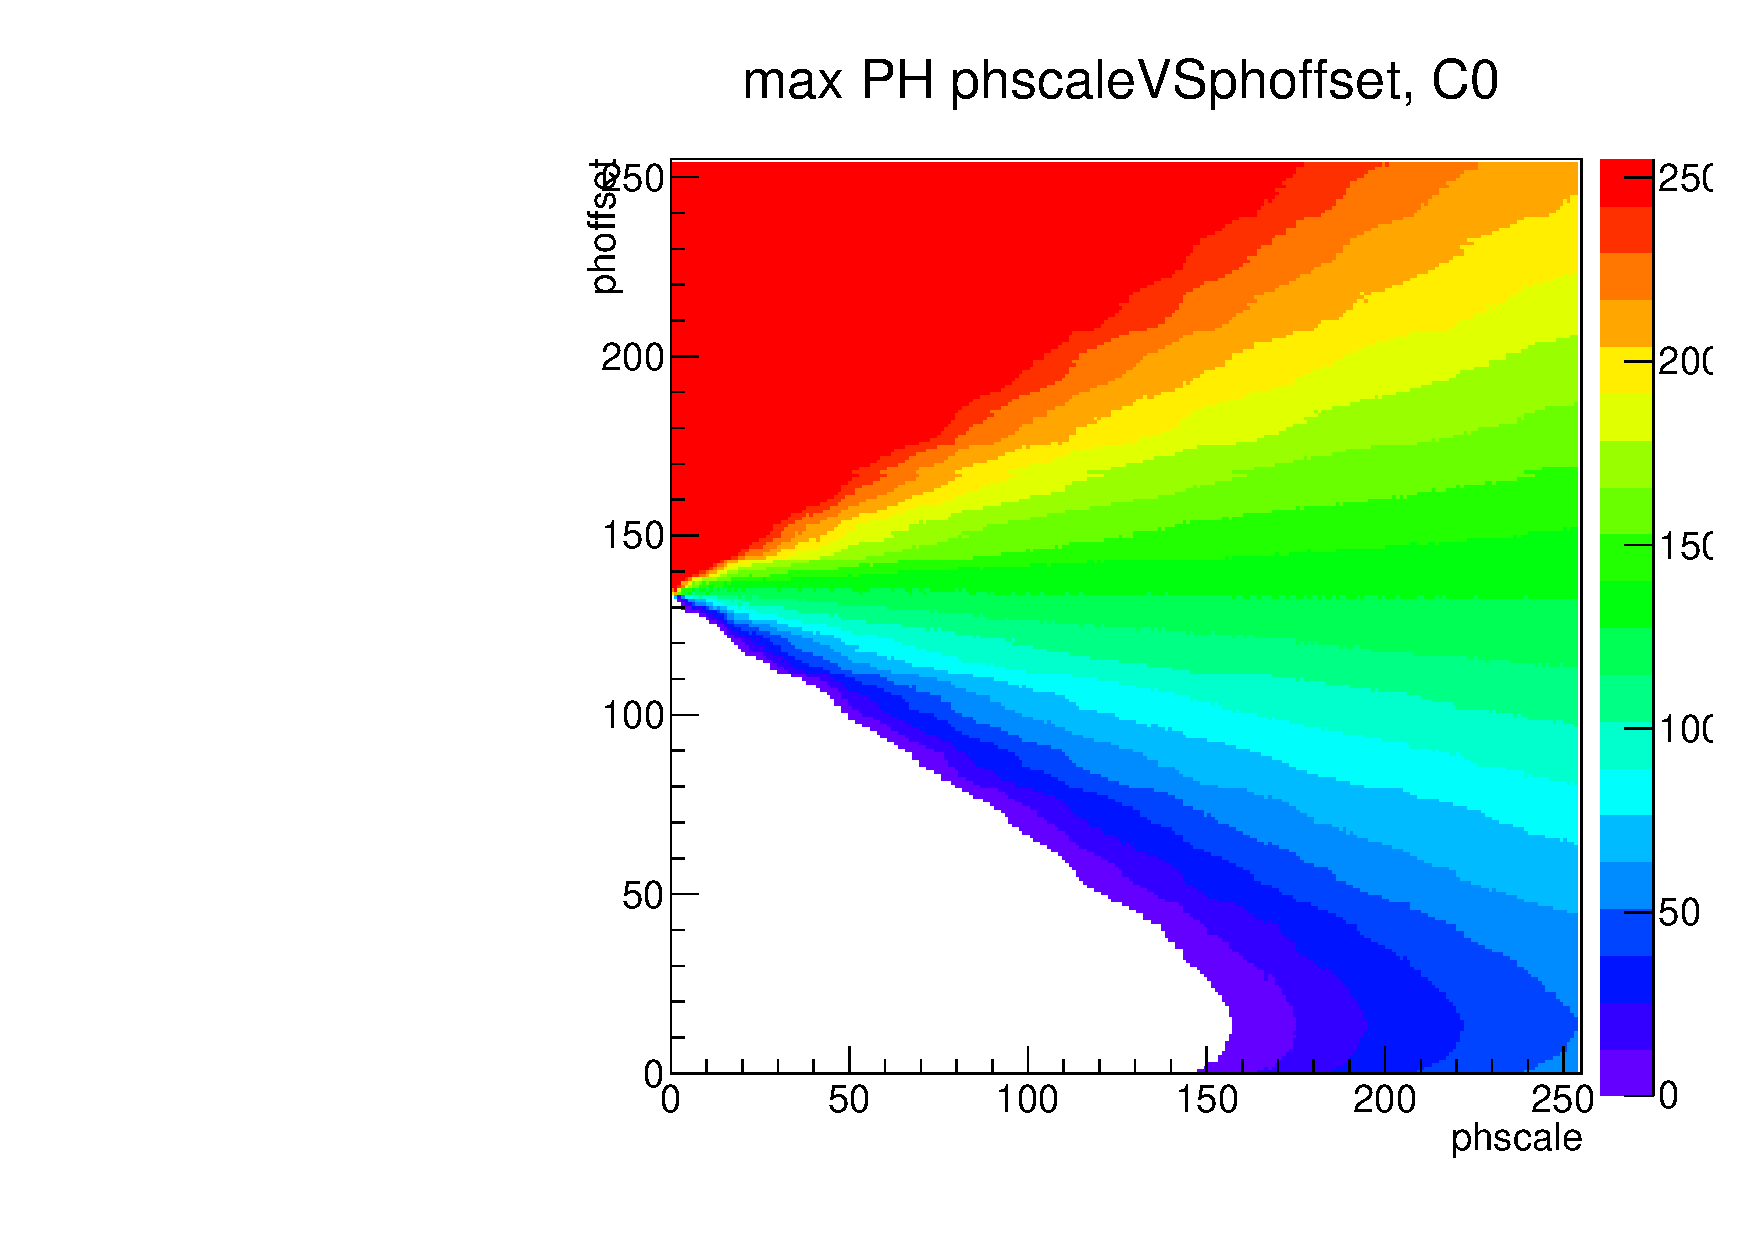
\includegraphics[width=1.0\textwidth]{figures/phopt_maxphvsdacdac_th2.pdf}
  \caption{}
  \label{fig:phopt_maxphvsdacdac_th2}
\end{minipage}
\end{figure}

\begin{figure}[!Hp]
\centering
\begin{minipage}{0.45\textwidth}
  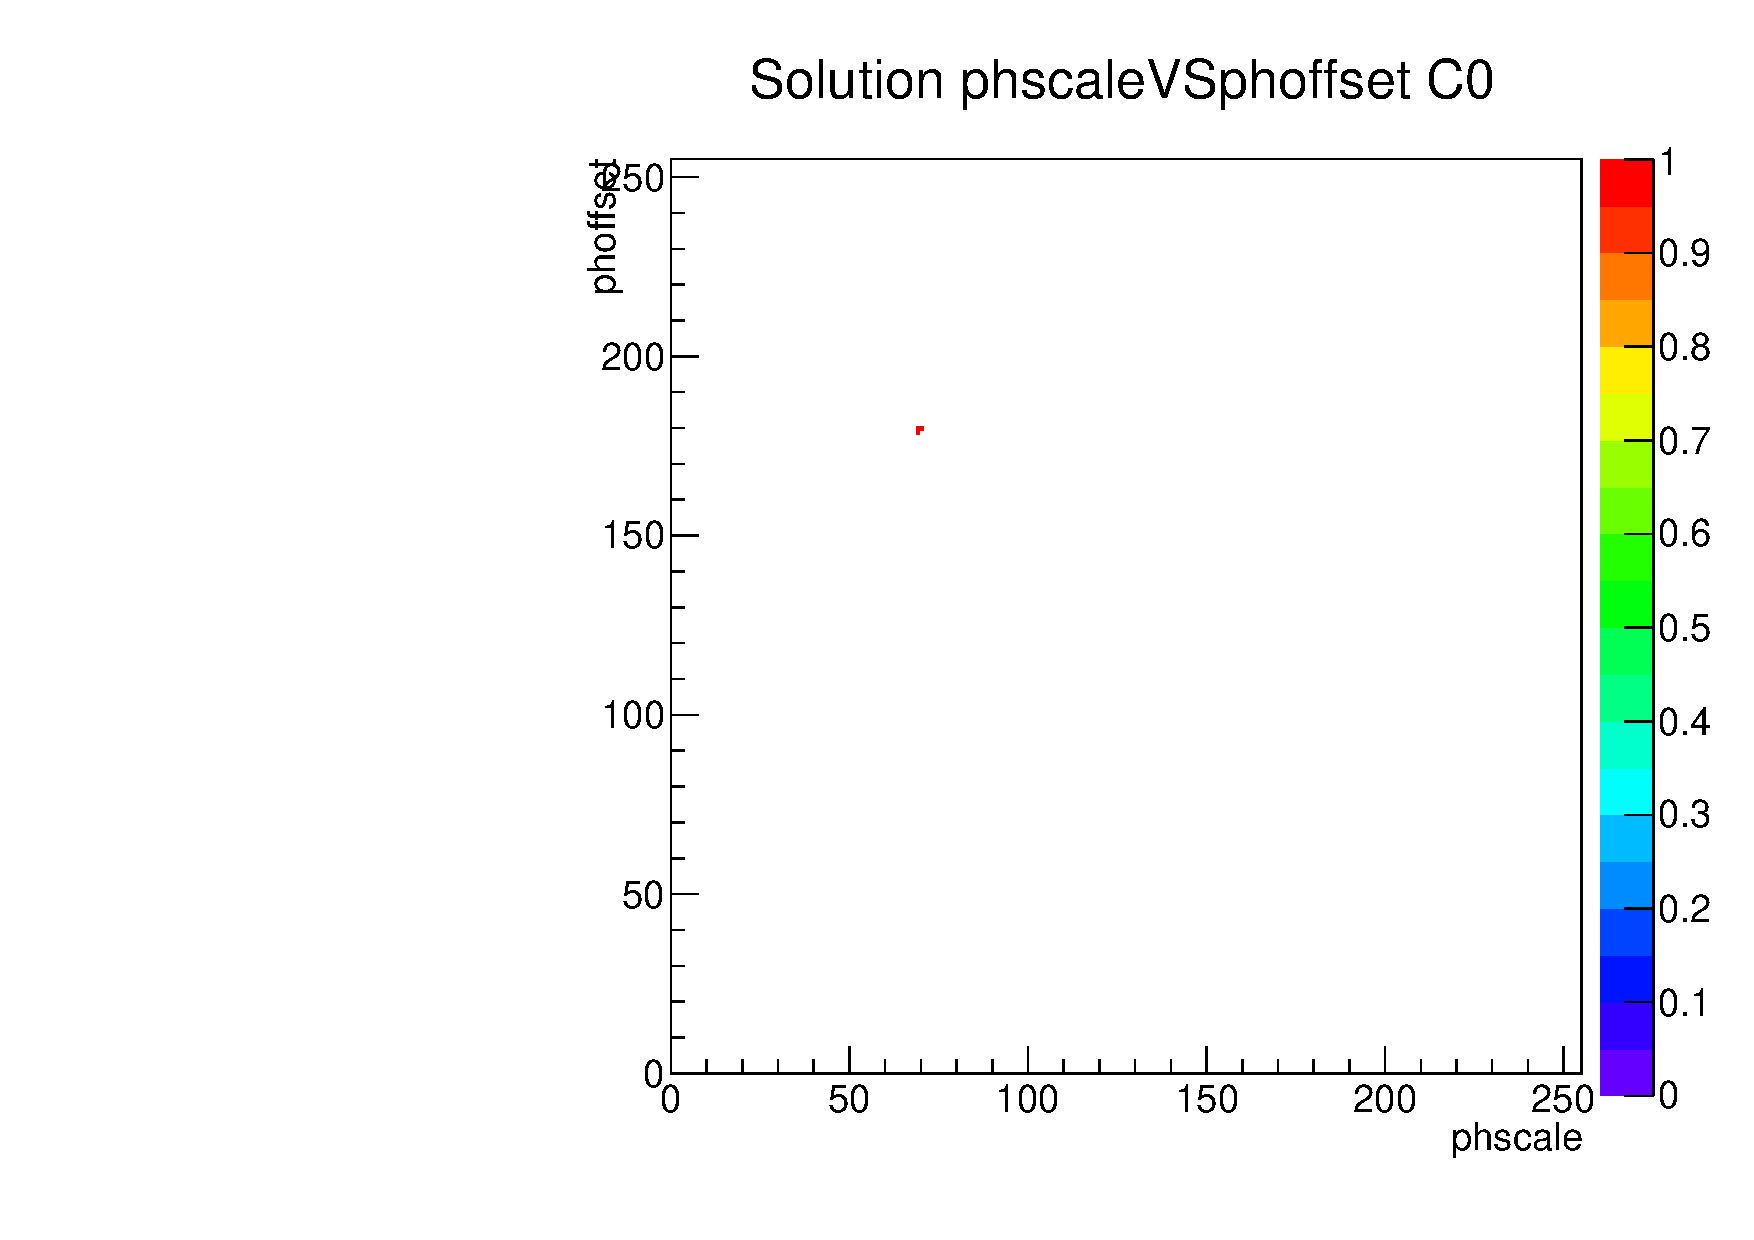
\includegraphics[width=1.0\textwidth]{figures/phopt_solphvsdacdac_th2.pdf}
  \caption{}
  \label{fig:phopt_solphvsdacdac_th2}
\end{minipage}
\end{figure}


% gain plots for highest/lowest gain pixels with optimized DACs

\begin{figure}[!Hp]
\centering
\begin{minipage}{0.45\textwidth}
  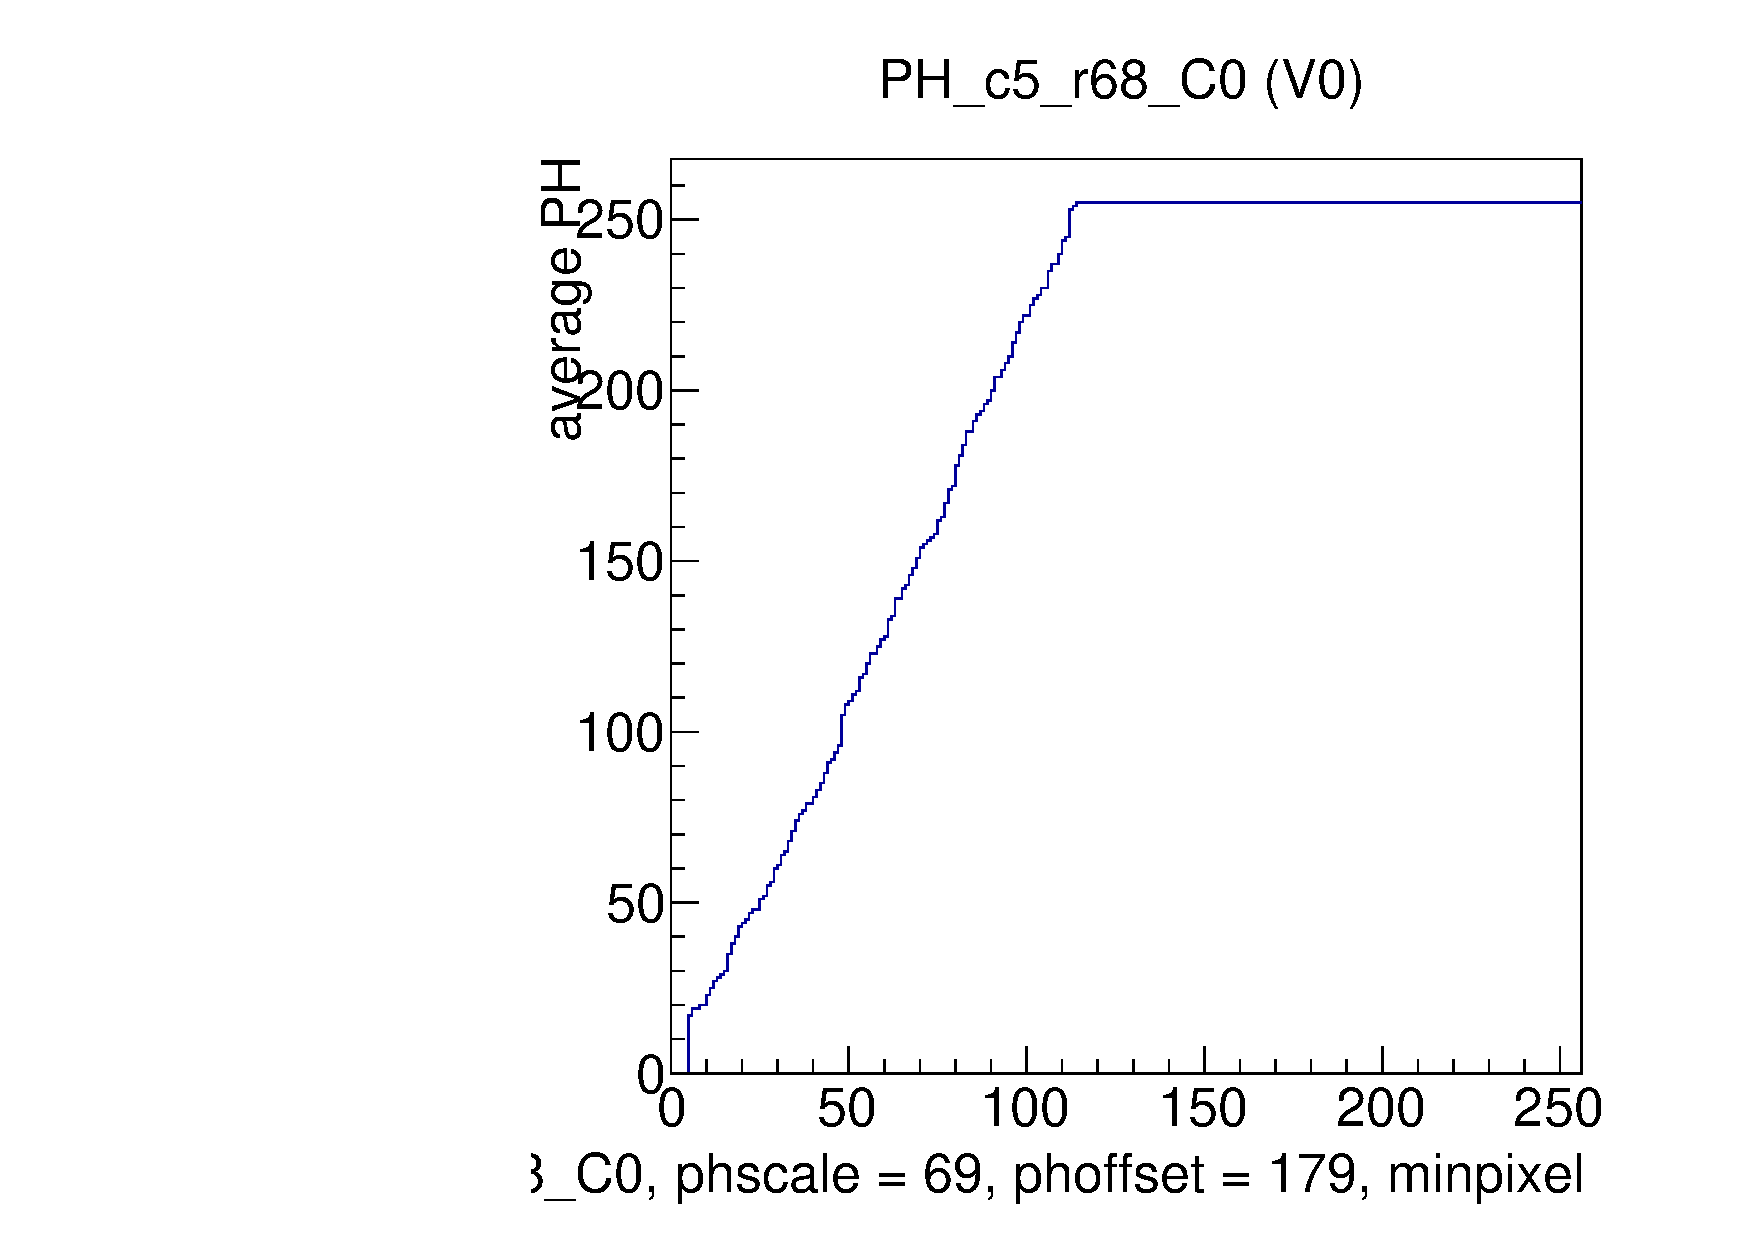
\includegraphics[width=1.0\textwidth]{figures/phopt_PH_c5_r68.pdf}
  \caption{}
  \label{fig:phopt_PH_c5_r68}
\end{minipage}
\hspace{0.3cm}
\begin{minipage}{0.45\textwidth}
  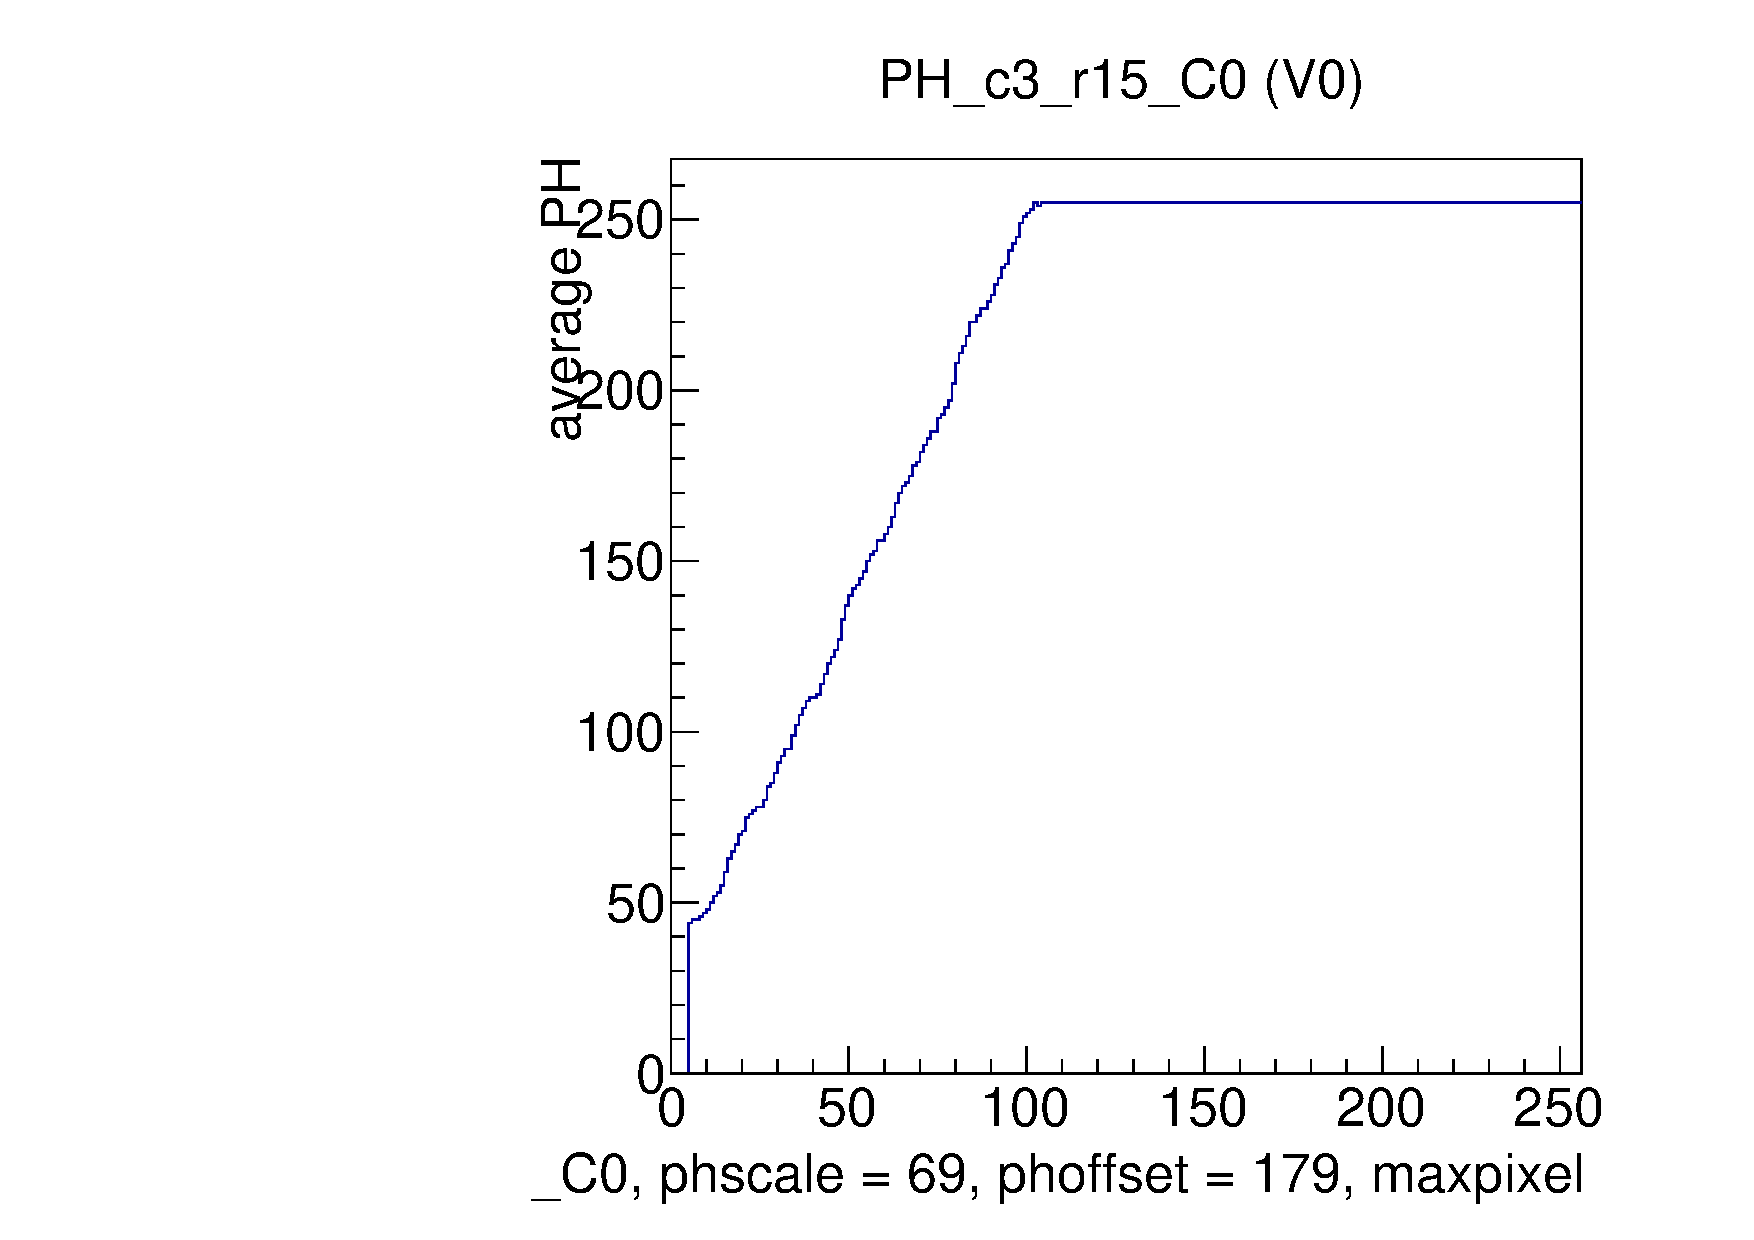
\includegraphics[width=1.0\textwidth]{figures/phopt_PH_c3_r15.pdf}
  \caption{}
  \label{fig:phopt_PH_c3_r15}
\end{minipage}
\end{figure}


% doing scans at three points in vcal

\begin{figure}[!Hp]
\centering
\begin{minipage}{0.45\textwidth}
  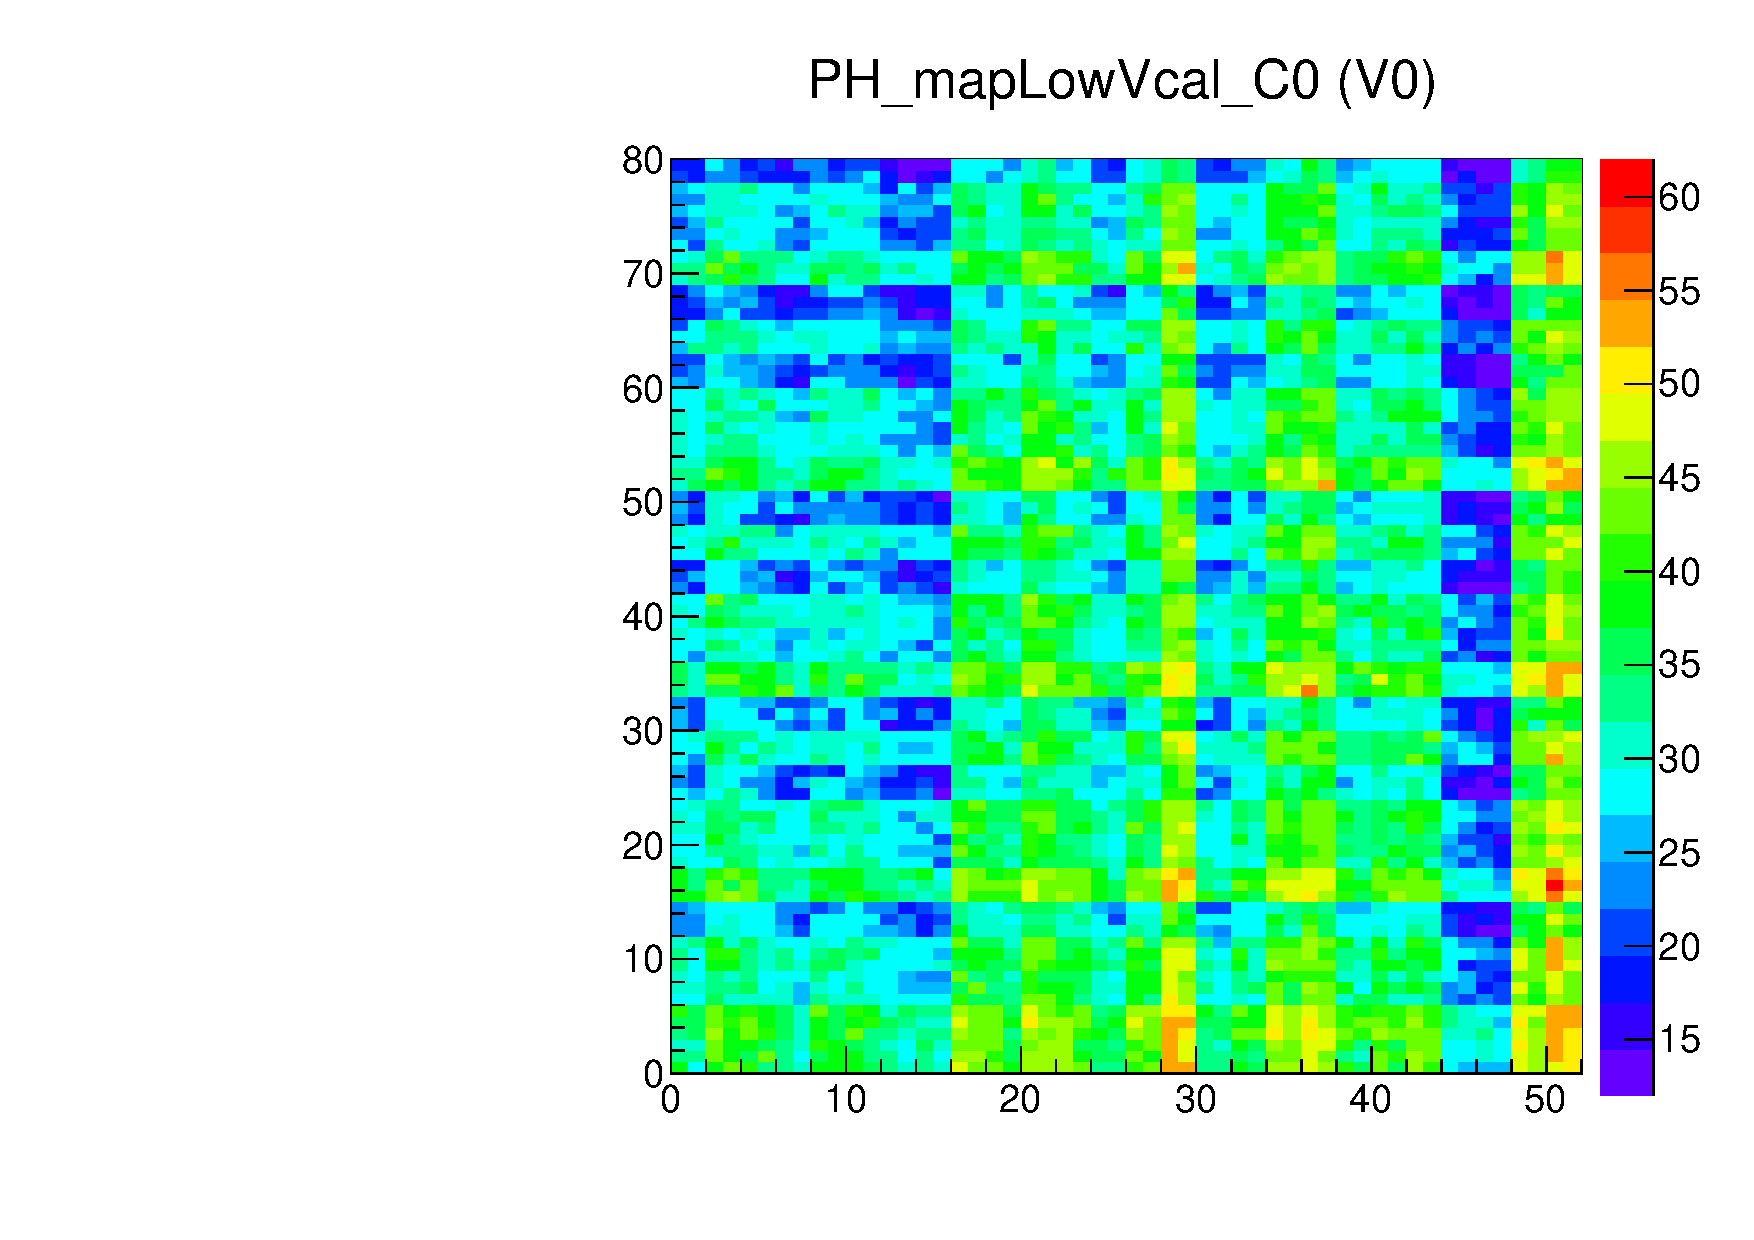
\includegraphics[width=1.0\textwidth]{figures/phopt_PH_mapLowVcal.pdf}
  \caption{}
  \label{fig:phopt_PH_mapLowVcal}
\end{minipage}
\hspace{0.3cm}
\begin{minipage}{0.45\textwidth}
  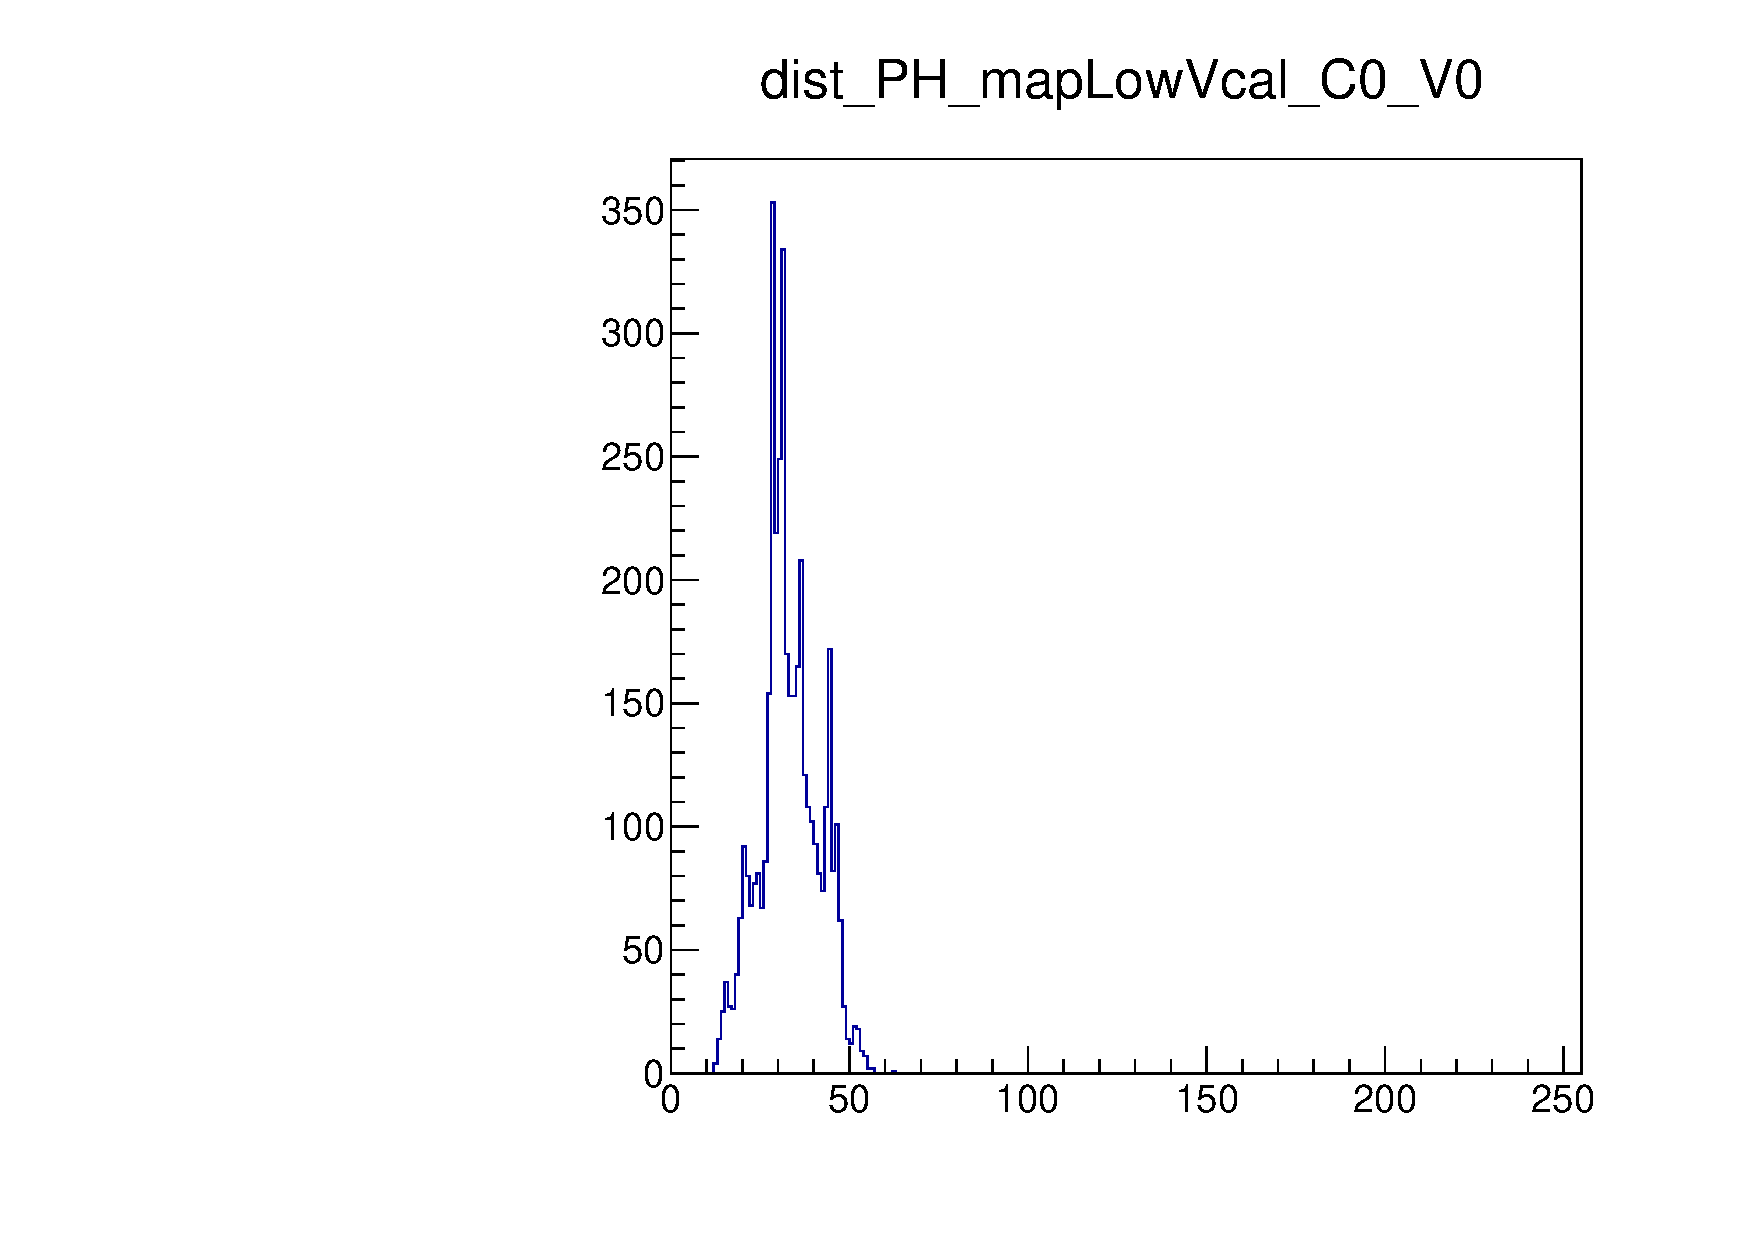
\includegraphics[width=1.0\textwidth]{figures/phopt_dist_PH_mapLowVcal.pdf}
  \caption{}
  \label{fig:phopt_dist_PH_mapLowVcal}
\end{minipage}
\end{figure}

\begin{figure}[!Hp]
\centering
\begin{minipage}{0.45\textwidth}
  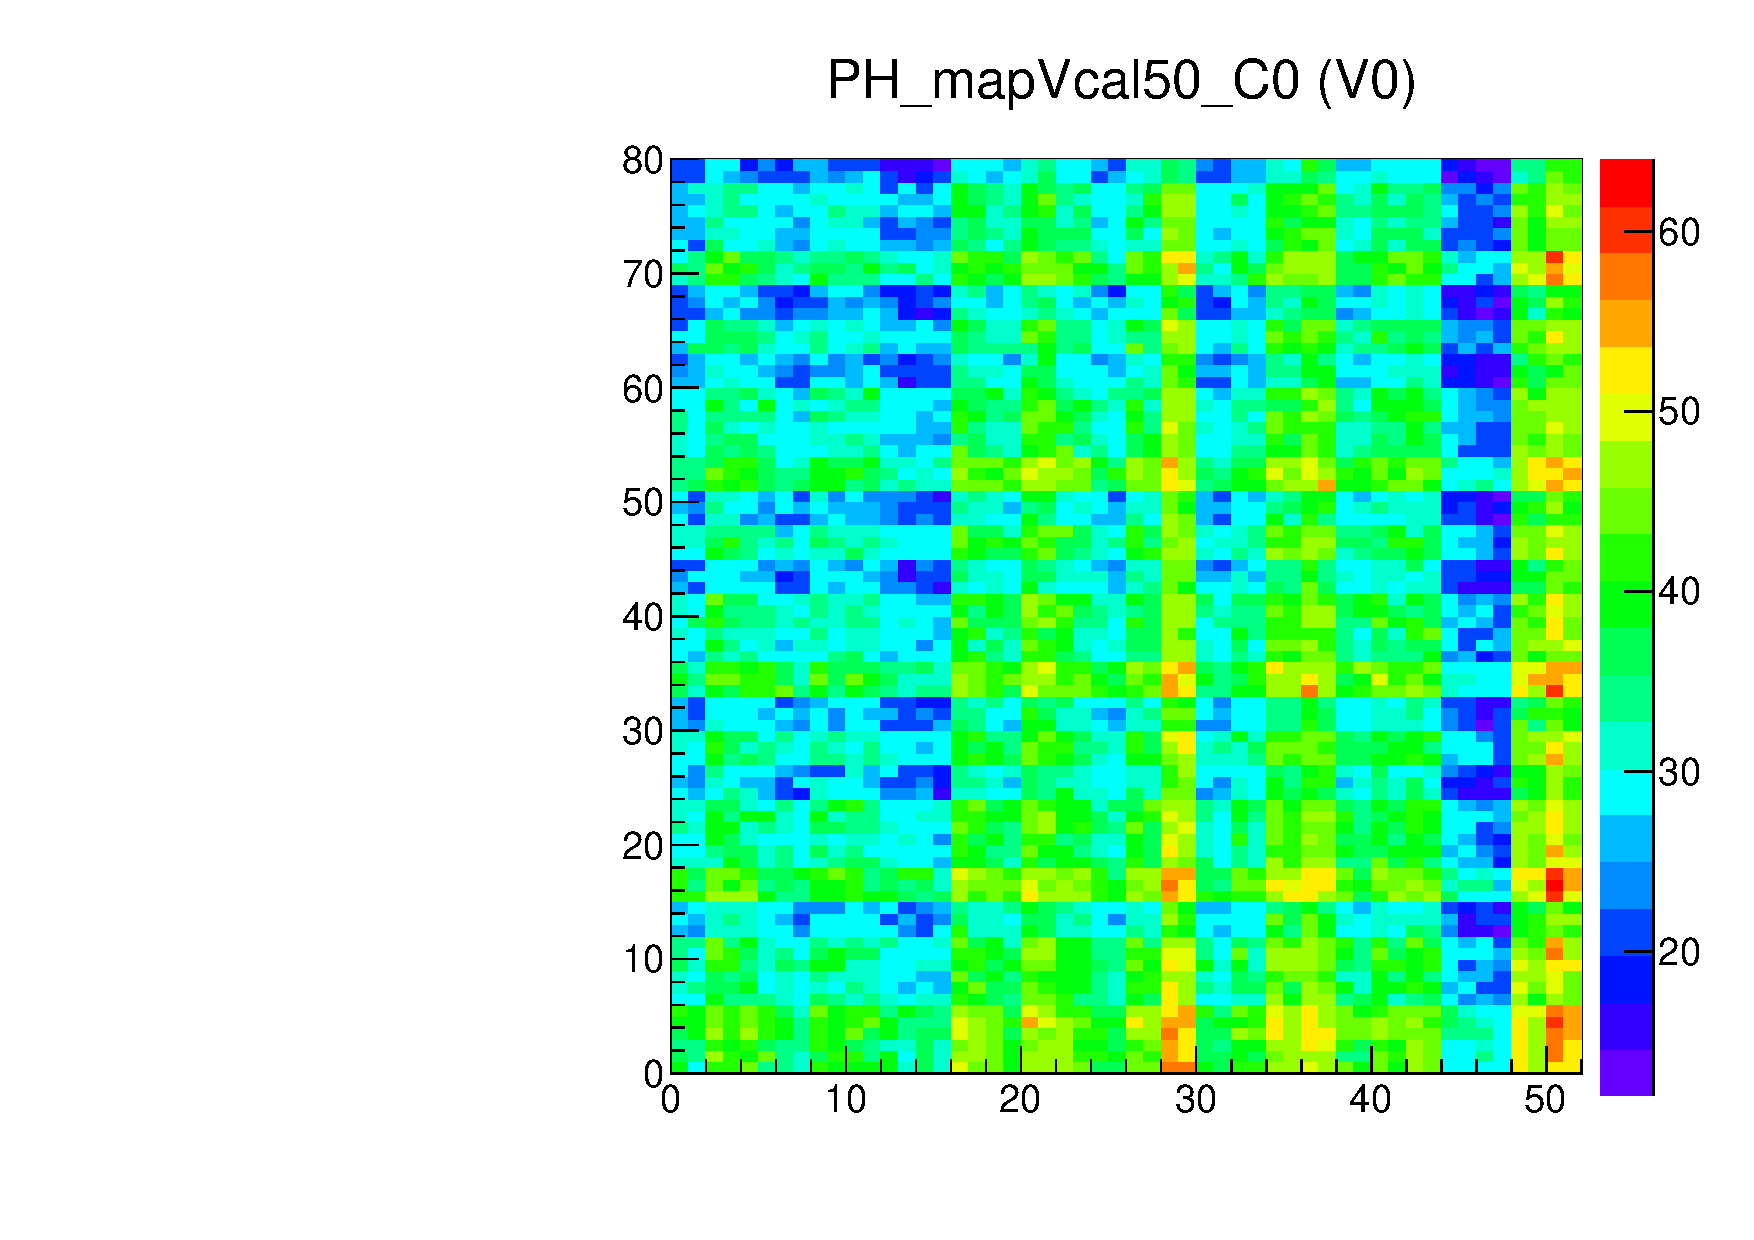
\includegraphics[width=1.0\textwidth]{figures/phopt_PH_mapVcal50.pdf}
  \caption{}
  \label{fig:phopt_PH_mapVcal50}
\end{minipage}
\hspace{0.3cm}
\begin{minipage}{0.45\textwidth}
  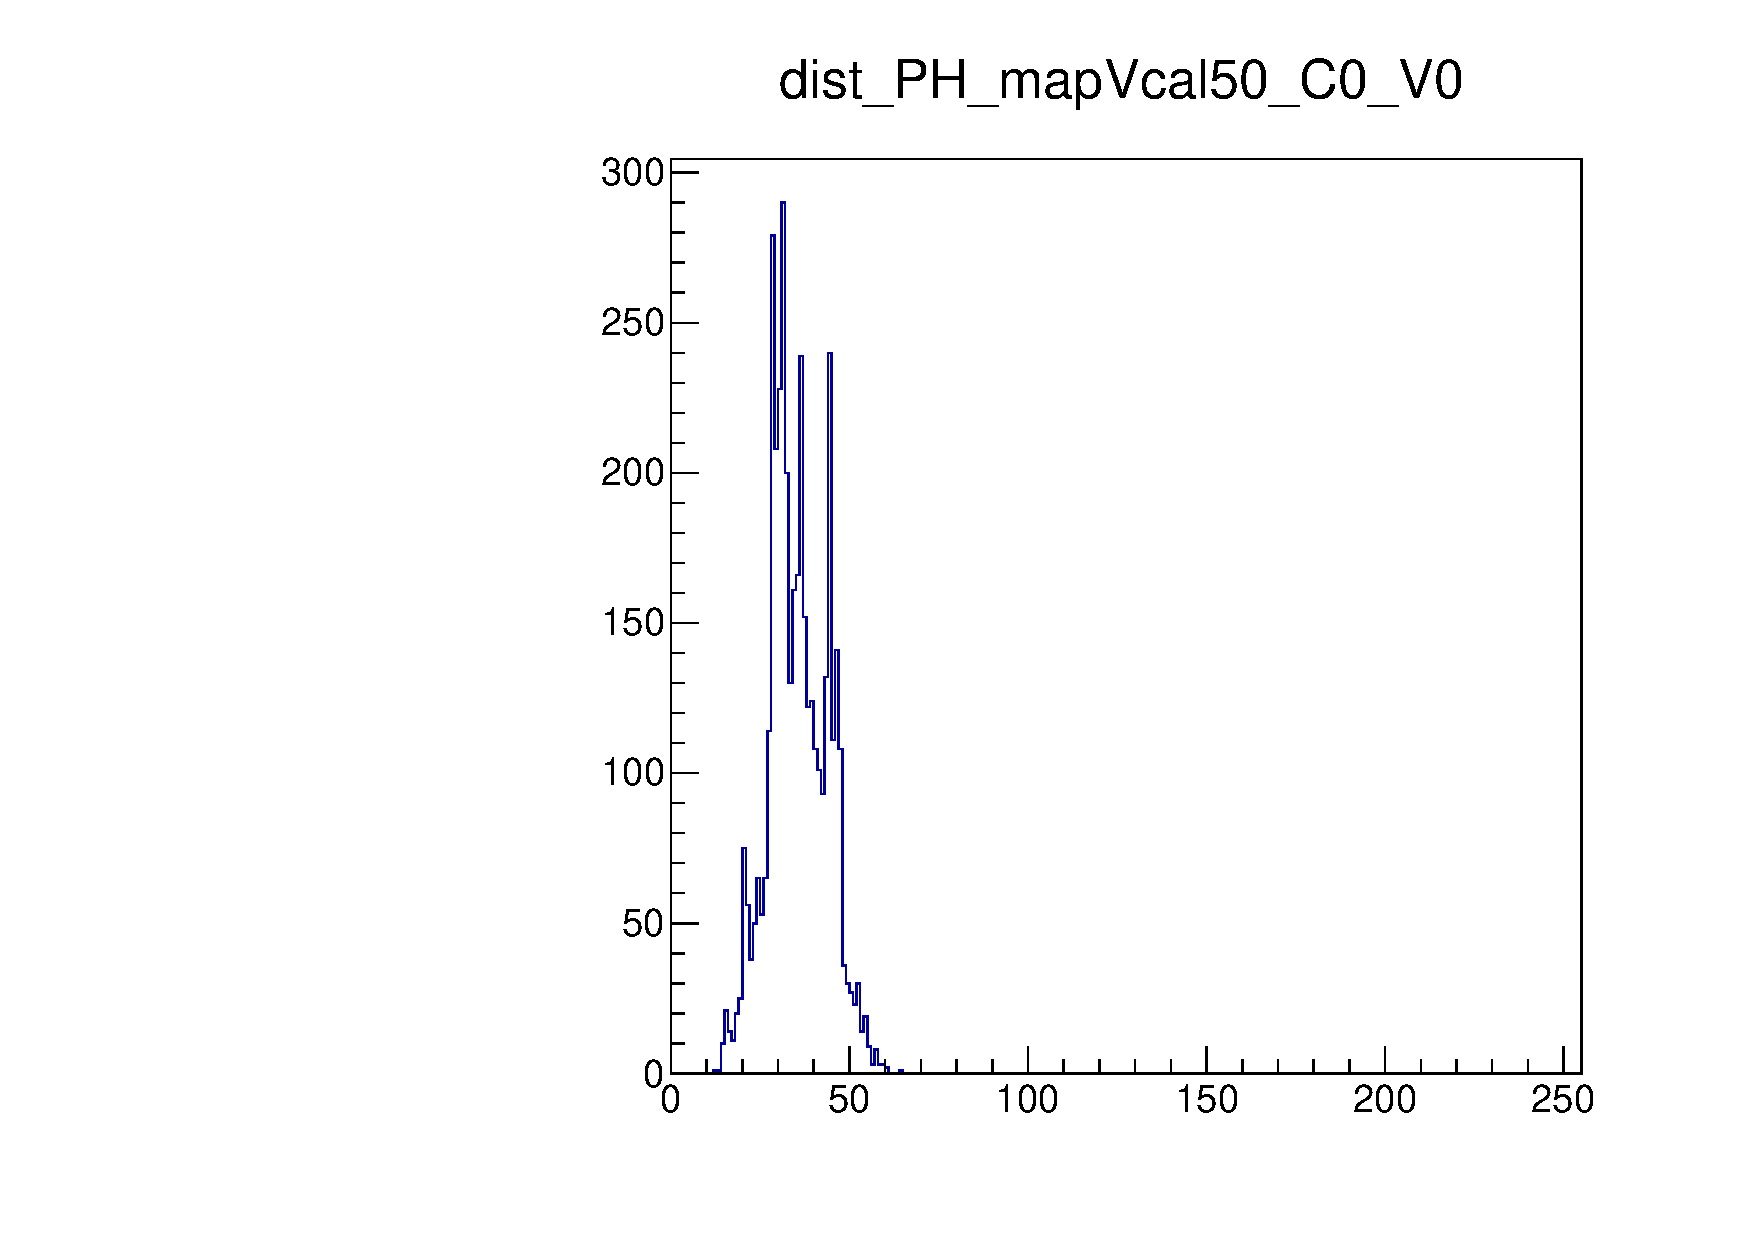
\includegraphics[width=1.0\textwidth]{figures/phopt_dist_PH_mapVcal50.pdf}
  \caption{}
  \label{fig:phopt_dist_PH_mapVcal50}
\end{minipage}
\end{figure}

\begin{figure}[!Hp]
\centering
\begin{minipage}{0.45\textwidth}
  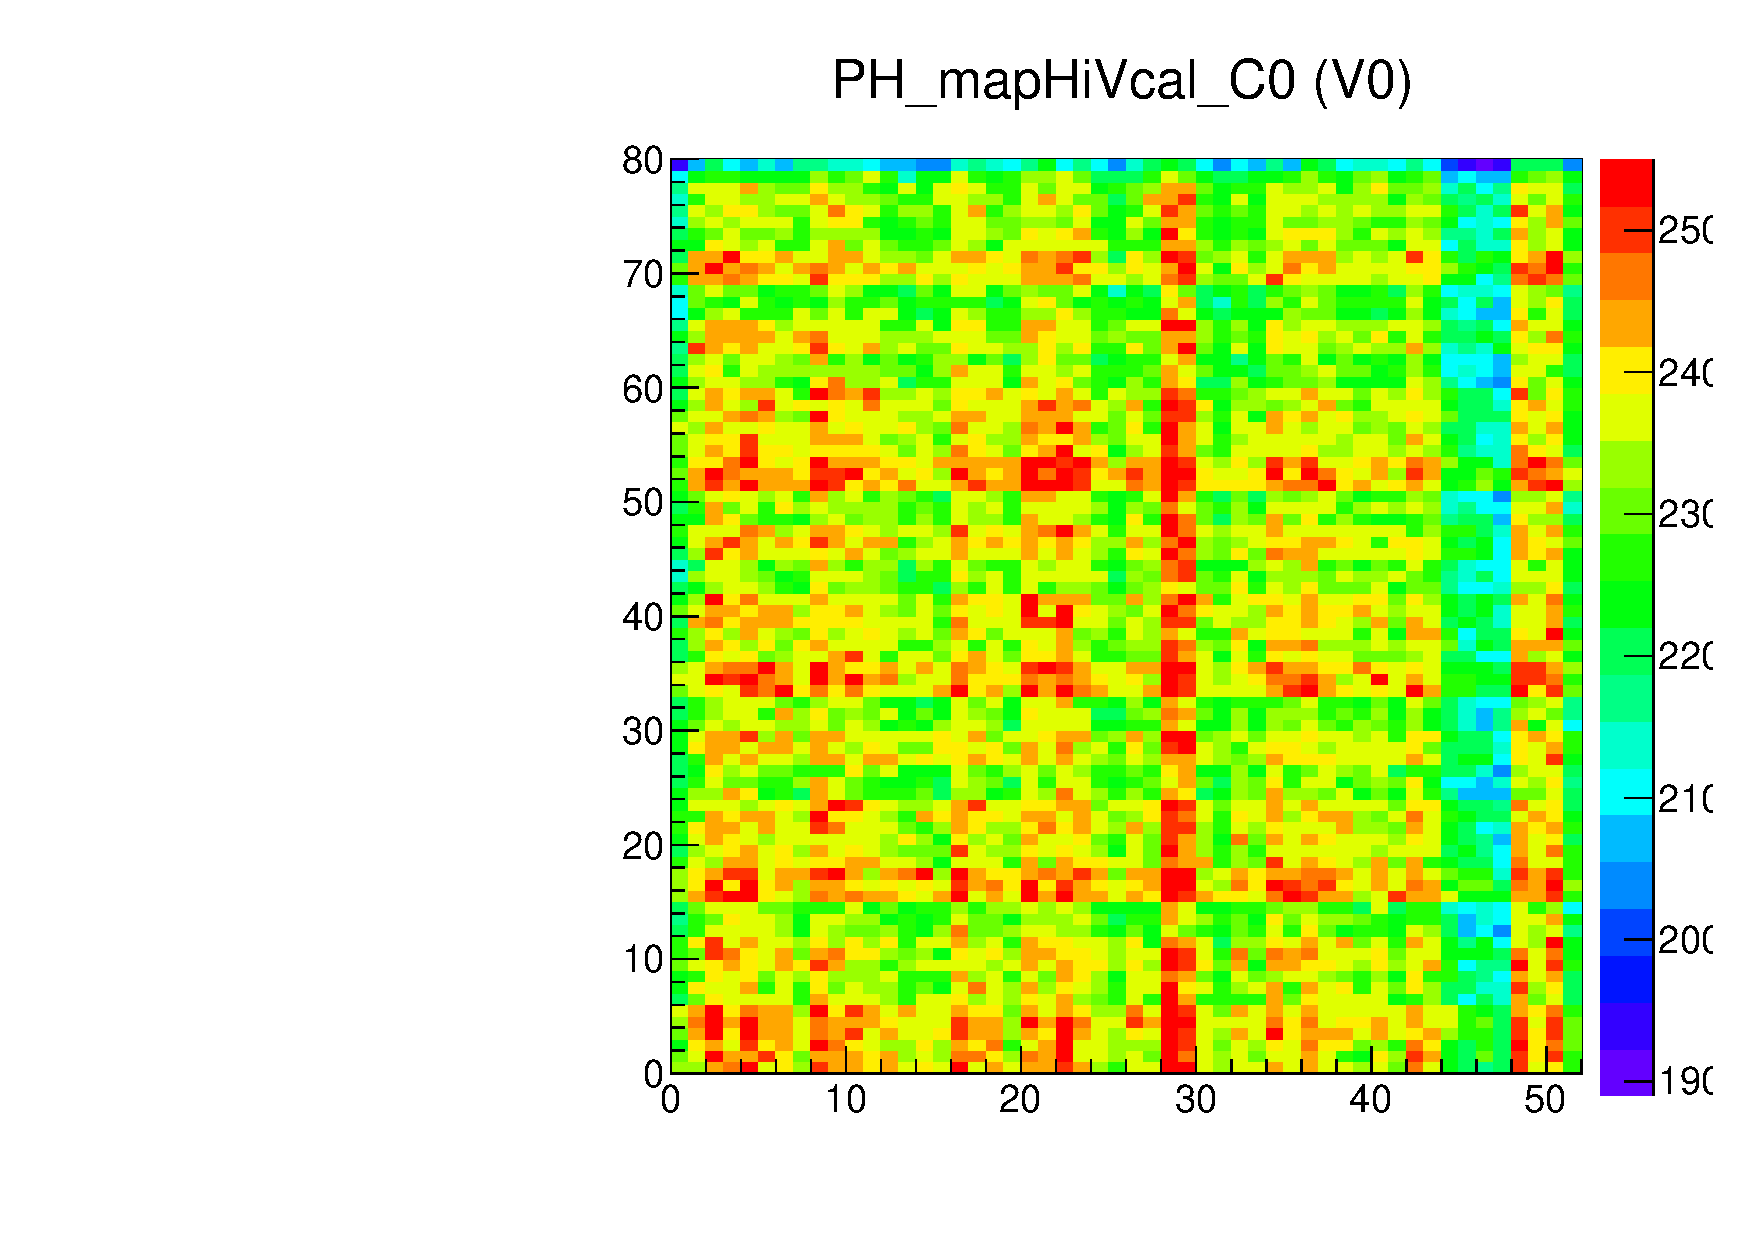
\includegraphics[width=1.0\textwidth]{figures/phopt_PH_mapHiVcal.pdf}
  \caption{}
  \label{fig:phopt_PH_mapHiVcal}
\end{minipage}
\hspace{0.3cm}
\begin{minipage}{0.45\textwidth}
  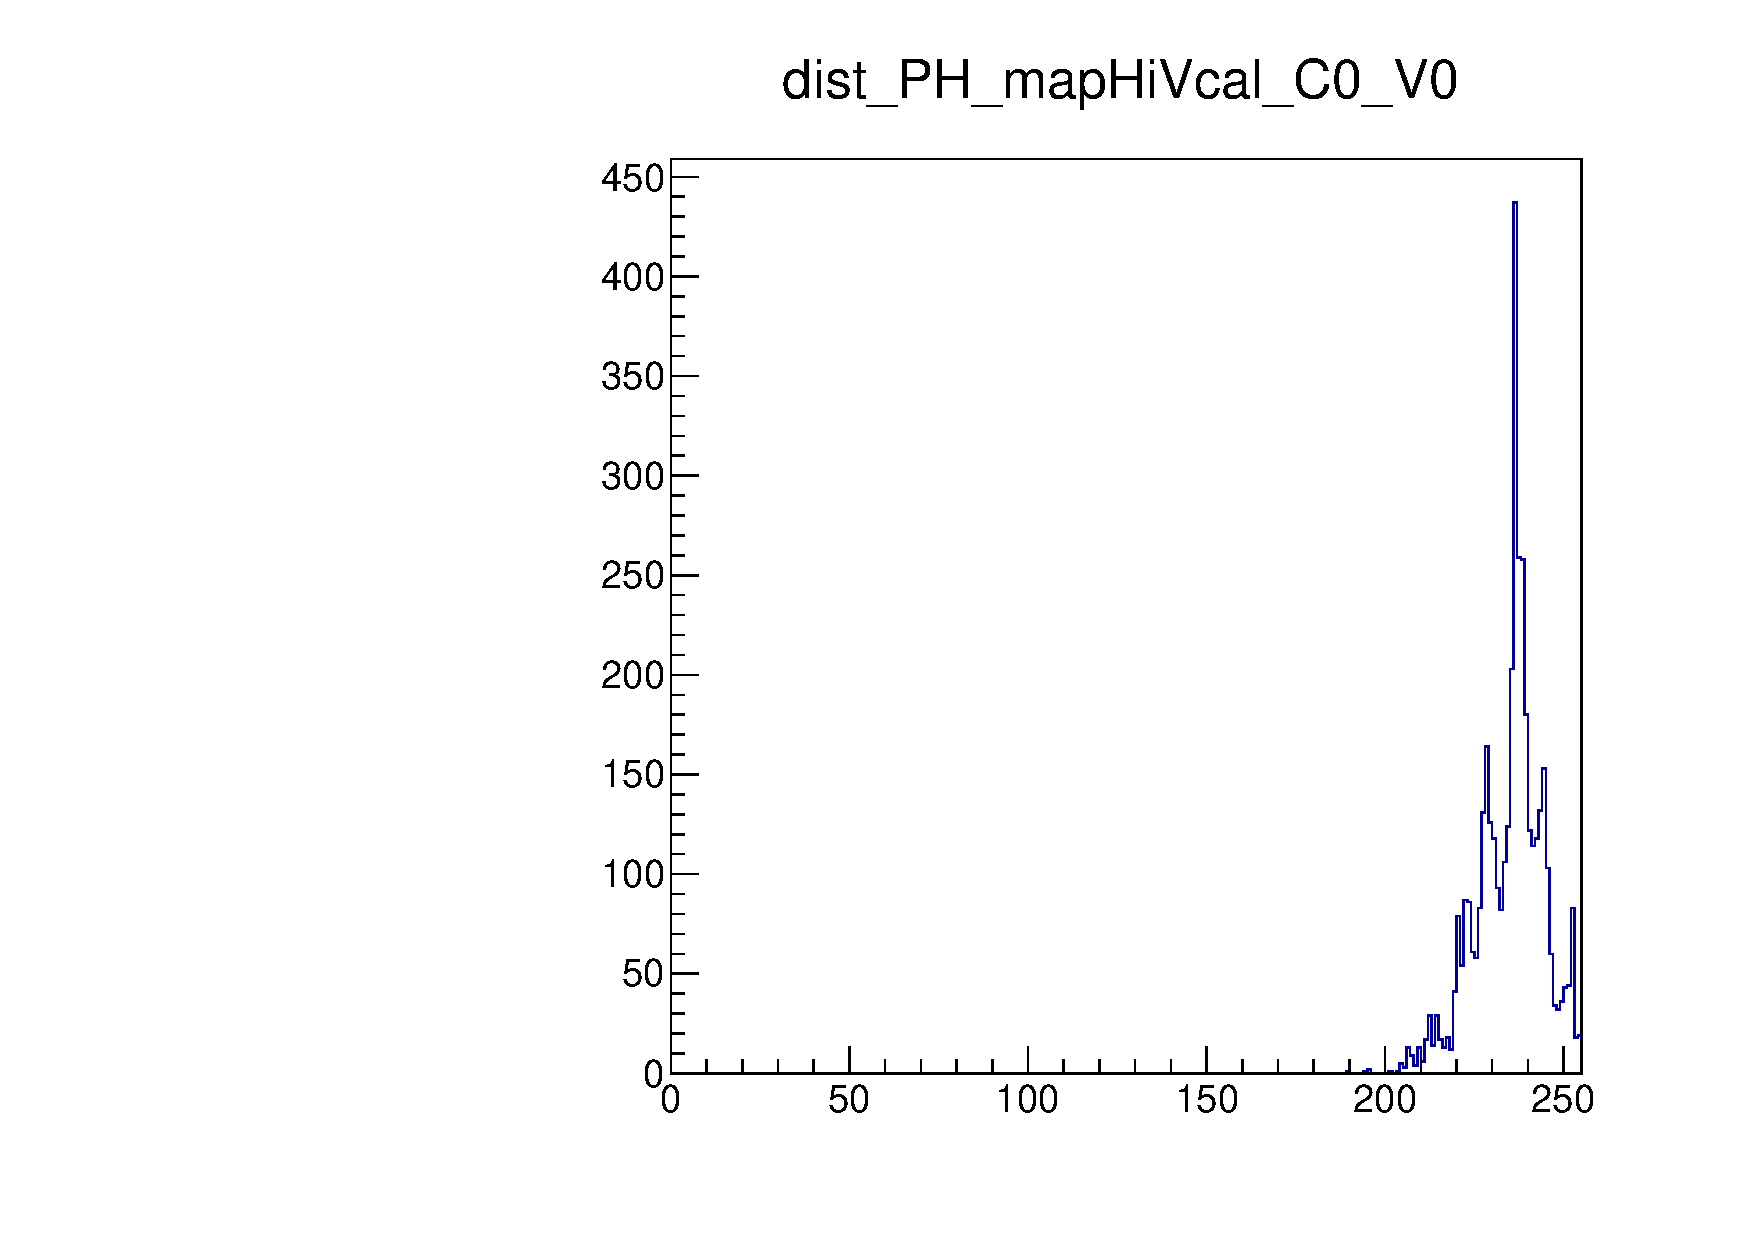
\includegraphics[width=1.0\textwidth]{figures/phopt_dist_PH_mapHiVcal.pdf}
  \caption{}
  \label{fig:phopt_dist_PH_mapHiVcal}
\end{minipage}
\end{figure}

